\section{Technical fundamentals}

This section will explain the technical fundamentals which are necessary to understand the full bachelor thesis.

\subsection{The Scapy library}

Scapy \cite{scapy} is a Python program that enables the user to send, sniff and dissect and forge network packets. This capability allows construction of tools that can probe, scan or attack networks.

It can be imagined similar to Wireshark, except that its usage happens in the terminal and not only allows reading network packets, but also crafting and sending them. It can also be used as a library by importing the necessary classes and interfaces into the own Python program. Scapy supports Python 3 and additionally Python 2, even though its support has ended on 1st of January 2020. The following quote from a maintainer explains the reason behind that:

\begin{displayquote}
    Scapy is a tool that can be used in a very large number of situations. Often, you don't get to choose the Python interpreter you have when you run Scapy. So, [...] we need to keep supporting Python 2.7 as long as we can.
\end{displayquote}

Understanding Scapy will be important for the later implementation in this work, since the UDS Scanner to be modified in this work is built within Scapy.

One of the core classes in Scapy is the \textbf{Packet} class. All definitions of network packet layers, such as Ethernet, IP, TCP, CAN, UDS and so on, are defined in a class inheriting from that class.

The well-known and simple UDP protocol \cite{udp} serves as an illustrative example.

For this it will be shown how the UDP header, shown in \autoref{fig:uds_header} is translated to such a Scapy class.

%UDP header
\begin{figure}[h]
    \centering
    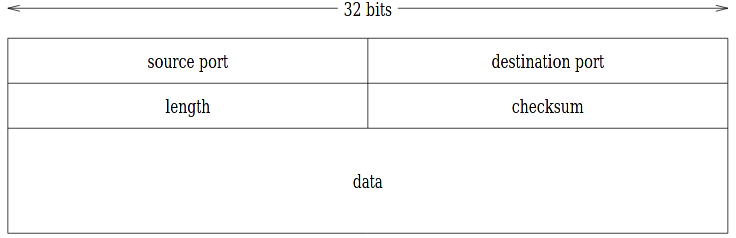
\includegraphics[width=0.7\textwidth]{udp_header}
    \caption{UDP header format \cite{udp_header}}
    \label{fig:uds_header}
\end{figure}

The UDP header format contains four fields and the data field. These four fields are translated literally into the Scapy class \textbf{UDP}. The data field is not part of it because Scapy uses an explicit operator to append data to the header information. This is shown later.

The following code snippet shows the explained class in the Scapy library.

\begin{minted}{python}
class UDP(Packet):
   fields_desc = [ShortEnumField("sport", 53, UDP_SERVICES),
                  ShortEnumField("dport", 53, UDP_SERVICES),
                  ShortField("len", None),
                  XShortField("chksum", None)]
\end{minted}

As in common programmer language, \textbf{short} specifies 16 bits. Since the UDP header only contains 16 bits fields, the Scapy definition only includes \textbf{short} fields. The first parameter of a field is always the name of this field. \textbf{sport} stands for source port, and \textbf{dport} for destination port.
The next parameter sets the default value for this field. This is defined by the Scapy programmers in all conscience and not by the official UDP standard. \textbf{53} specifies the DNS protocol.
\textbf{EnumField}s also contain a third argument. This is a simple dictionary mapping from machine-readable values to human-readable texts. For example, part of the \textbf{UDP\_SERVICES} dictionary is: \mintinline{python}{{53: "domain", 80: "www_http"}}
The following snippets shows some examples of how to instantiate an object of the UDP class and also demonstrates how to append data to the headers with the “/” operator.

\begin{minted}{python}
packet = UDP(dport=80) # is equivalent to:
packet = UDP(dport="www_http")

# Append 0x00 as data
packet = UDP(dport=80) / Raw(b'\x00')
\end{minted}

Now it shall be explained, how to actually send a packet and receive a response. For this, a socket is required. Scapy provides many kinds of sockets for different use cases. For example the \textbf{L2Socket} and the \textbf{L3PacketSocket}. The difference between them is that L2Socket expects a packet object containing all information starting from Ethernet (Layer 2), while L3PacketSocket expected a packet object only containing all information starting from IP (layer 3). The following code snippet uses the L2Socket for full coverage of the whole packet stack and explains how sending and receiving of a packet works (Note: Root privileges might be necessary for this to work):

\begin{minted}{python}
# import necessary classes
from scapy.arch.linux import L2Socket
# Create a layer 2 socket specifing the interface name
socket = L2Socket("eth0")
# Create a packet covering layer 2 to 7, targeting the Google server
# This packet starts a TCP handshake, thus the SYN flag is exclusively set
# Set destination port to HTTP and a high source port
packet = Ether() / IP(dst="142.250.185.163") / TCP(flags="S", dport=80, sport=60123)
# sr1 stands for: send receive one
# it sends the given packet and returns the response
response = socket.sr1(packet)
# This displays the response in a human-friendly form
response.show()
\end{minted}

The .show() command gives the following output. It has been slightly edited to be more compact and some information has been replaced by placeholders for privacy reasons.

\begin{minted}{text}
###[ Ethernet ]### 
  dst       = 12:34:45:67:89:ab
  src       = 2c:3a:fd:af:64:e0
  type      = IPv4
###[ IP ]### 
     version   = 4
     src       = 142.250.185.163
     dst       = 123.123.123.123
###[ TCP ]### 
        sport     = www_http
        dport     = 60123
        flags     = SA
\end{minted}

The SYN and ACK flags are set now as expected for the TCP handshake. Furthermore, the dport of the response is the sport of the request.


\subsection{The UDS protocol}

\subsection{The UDS Scanner}
